\documentclass{standalone}
\usepackage{graphicx}	
\usepackage{amssymb, amsmath}
\usepackage{color}

\usepackage{tikz}
\usetikzlibrary{intersections, backgrounds, math}
\usepackage{pgfmath}

\definecolor{light}{RGB}{220, 188, 188}
\definecolor{mid}{RGB}{185, 124, 124}
\definecolor{dark}{RGB}{143, 39, 39}
\definecolor{highlight}{RGB}{180, 31, 180}
\definecolor{gray10}{gray}{0.1}
\definecolor{gray20}{gray}{0.2}
\definecolor{gray30}{gray}{0.3}
\definecolor{gray40}{gray}{0.4}
\definecolor{gray60}{gray}{0.6}
\definecolor{gray70}{gray}{0.7}
\definecolor{gray80}{gray}{0.8}
\definecolor{gray90}{gray}{0.9}
\definecolor{gray95}{gray}{0.95}

\begin{document}

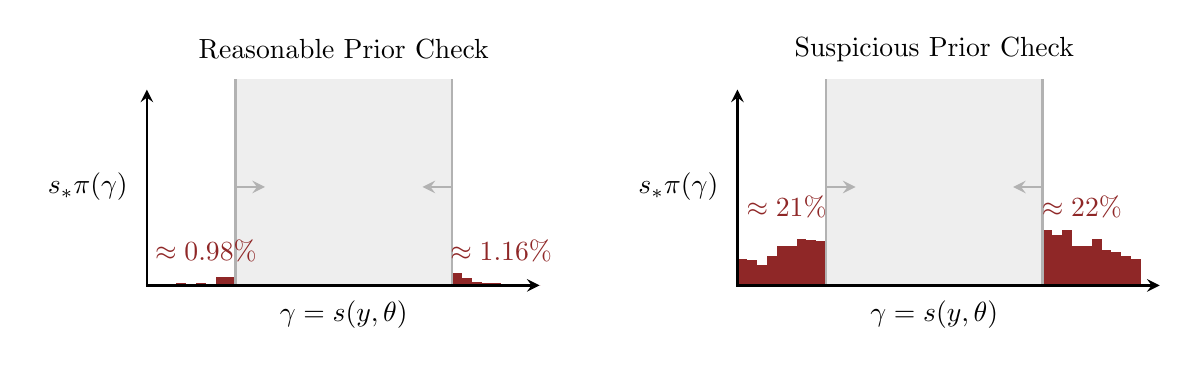
\begin{tikzpicture}[scale=0.25, thick]

  
  \begin{scope}[shift={(0, 0)}]
    \draw[white] (-16, -3) rectangle (12, 13);
    
    \node at (0, 12) { Reasonable Prior Check };
  
    \fill[color=gray80, opacity=0.33] (-5.5, 0) rectangle (5.5, 10.5);
    
    \foreach[count=\n] \y in {0.000, 0.000, 1.000, 4.000, 2.000, 5.000, 3.000, 17.000, 17.000} {
      \fill[dark] ({(\n - 1) / 2 - 10}, 0) rectangle ({(\n) / 2 - 10}, {0.025 * \y});
    }
    
    \foreach[count=\n] \y in {25.000, 15.000, 6.000, 5.000, 5.000, 0.000, 2.000, 0.000, 0.000} {
      \fill[dark] ({(\n + 31 - 1) / 2 - 10}, 0) rectangle ({(\n + 31) / 2 - 10}, {0.025 * \y});
    }
    
    \draw[-, color=gray70, line width=1] (-5.5, 0) -- (-5.5, 10.5);
    \draw[->, >=stealth, line width=1, color=gray70] (-5.5, 5) -- +(1.5, 0);
  
    \draw[-, color=gray70, line width=1] (5.5, 0) -- (5.5, 10.5);
    \draw[->, >=stealth, line width=1, color=gray70] (5.5, 5) -- +(-1.5, 0);
  
    \draw [->, >=stealth, line width=1] (-10.00, -0.05) -- +(0, 10);
    \draw [->, >=stealth, line width=1] (-10.05, +0.00) -- +(20, 0);
    
    \node[dark] at (-7, 1.75) { $\approx 0.98\%$ };
    \node[dark] at (+8, 1.75) { $\approx 1.16\%$ };
    
    \node[] at (-13, 5) { $s_{*} \pi(\gamma)$ };
    \node[] at (0, -1.5) { $\gamma = s(y, \theta)$ };
  \end{scope}
  
  \begin{scope}[shift={(30, 0)}]
    \draw[white] (-16, -3) rectangle (12, 13);
    
    \node at (0, 12) { Suspicious Prior Check };
  
    \fill[color=gray80, opacity=0.33] (-5.5, 0) rectangle (5.5, 10.5);
    
    \foreach[count=\n] \y in {54.000, 52.000, 41.000, 60.000, 81.000, 80.000, 95.000, 92.000, 91.000} {
      \fill[dark] ({(\n - 1) / 2 - 10}, 0) rectangle ({(\n) / 2 - 10}, {0.025 * \y});
    }
    
    \foreach[count=\n] \y in {113.000, 102.000, 113.000, 80.000, 80.000, 94.000, 71.000, 67.000, 59.000, 53.000} {
      \fill[dark] ({(\n + 31 - 1) / 2 - 10}, 0) rectangle ({(\n + 31) / 2 - 10}, {0.025 * \y});
    }
    
    \draw[-, color=gray70, line width=1] (-5.5, 0) -- (-5.5, 10.5);
    \draw[->, >=stealth, line width=1, color=gray70] (-5.5, 5) -- +(1.5, 0);
  
    \draw[-, color=gray70, line width=1] (5.5, 0) -- (5.5, 10.5);
    \draw[->, >=stealth, line width=1, color=gray70] (5.5, 5) -- +(-1.5, 0);
  
    \draw [->, >=stealth, line width=1] (-10.00, -0.05) -- +(0, 10);
    \draw [->, >=stealth, line width=1] (-10.05, +0.00) -- +(21.5, 0);
    
    \node[dark] at (-7.5, 4) { $\approx 21\%$ };
    \node[dark] at (+7.5, 4) { $\approx 22\%$ };
    
    \node[] at (-13, 5) { $s_{*} \pi(\gamma)$ };
    \node[] at (0, -1.5) { $\gamma = s(y, \theta)$ };
  \end{scope}
  
\end{tikzpicture}

\end{document}  